\documentclass[12pt]{article}
\usepackage{graphicx}

\author{Samuel Young}
\title{Exam II question II}
\date{Thursday November 24th, 2018}
\begin{document}
\maketitle

\part{2.A}
   There are just about 72 possible ALL and AML data point within the data set. There are a total 47 ALL in the dataset and 25 of the AML in the same data set. So the genes are the rows and the columns are the patients. So first I did a wordcount on the file to see how many rows there are and then minus the 7219-1 to get a close approximation to the numbers there are 72* 7218 differnet genes to look at for the data set.
 
  \part{2.B}
   I've  put it throught the algorithum multply times have recieved there is about 3934000-3936999 of them that are less than .05 that at the intial p-value. In all cases there is something like 721800 possible there is about half of the time shuffle are less or .05=$\alpha$ 
                 
\part{2.C}
    So each curve is bases on the intial thousand that is created within the simulated t values. The reason for this is to keep it simpilicity and it will also vary within each shuffled version of the graph. Because of t obsevered is negative value there must also be a another positive value to balance out the curve. There is probabilty at least one graph that has siginificantly lowerer the $\alpha$.
                  \begin{figure}
                  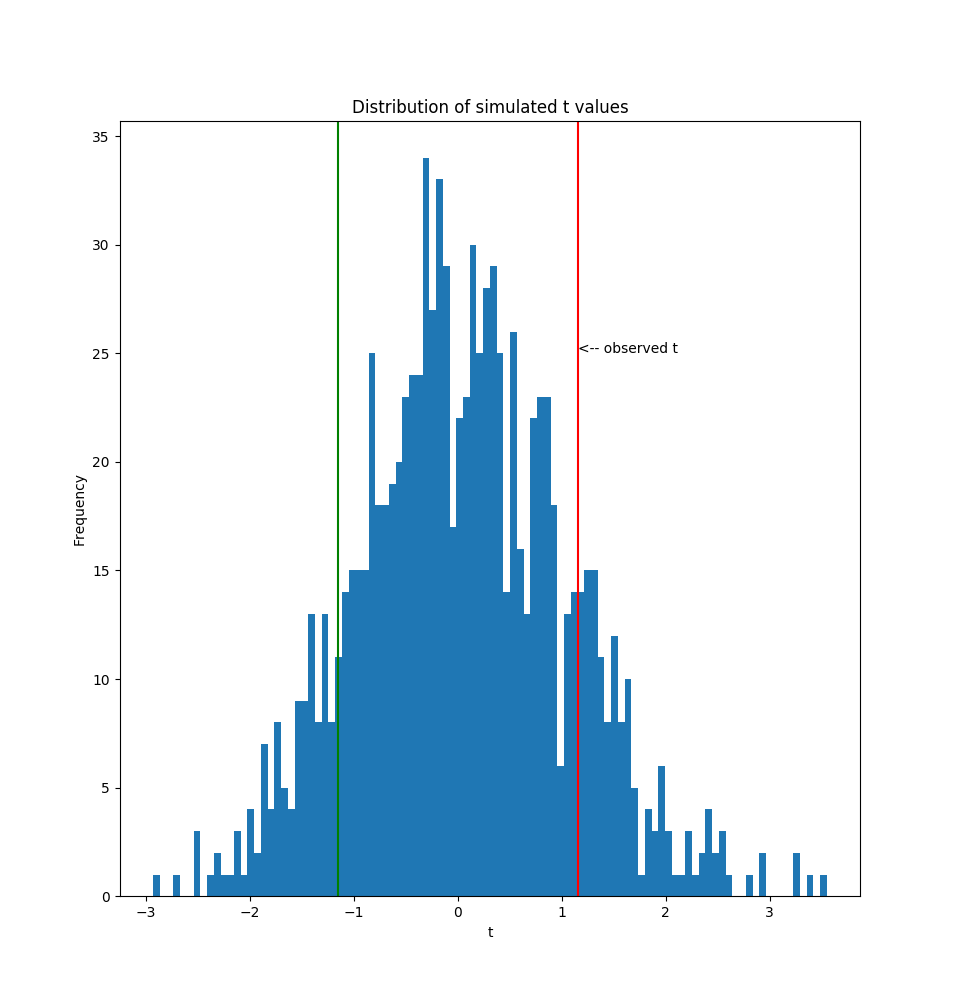
\includegraphics[width=\linewidth]{./Figure-1.png}
                  \caption{They are two side bell-like-curves with the observed t in red and green.}
                  \label{fig:graph1}
                  \end{figure}

                 \begin{figure}
                 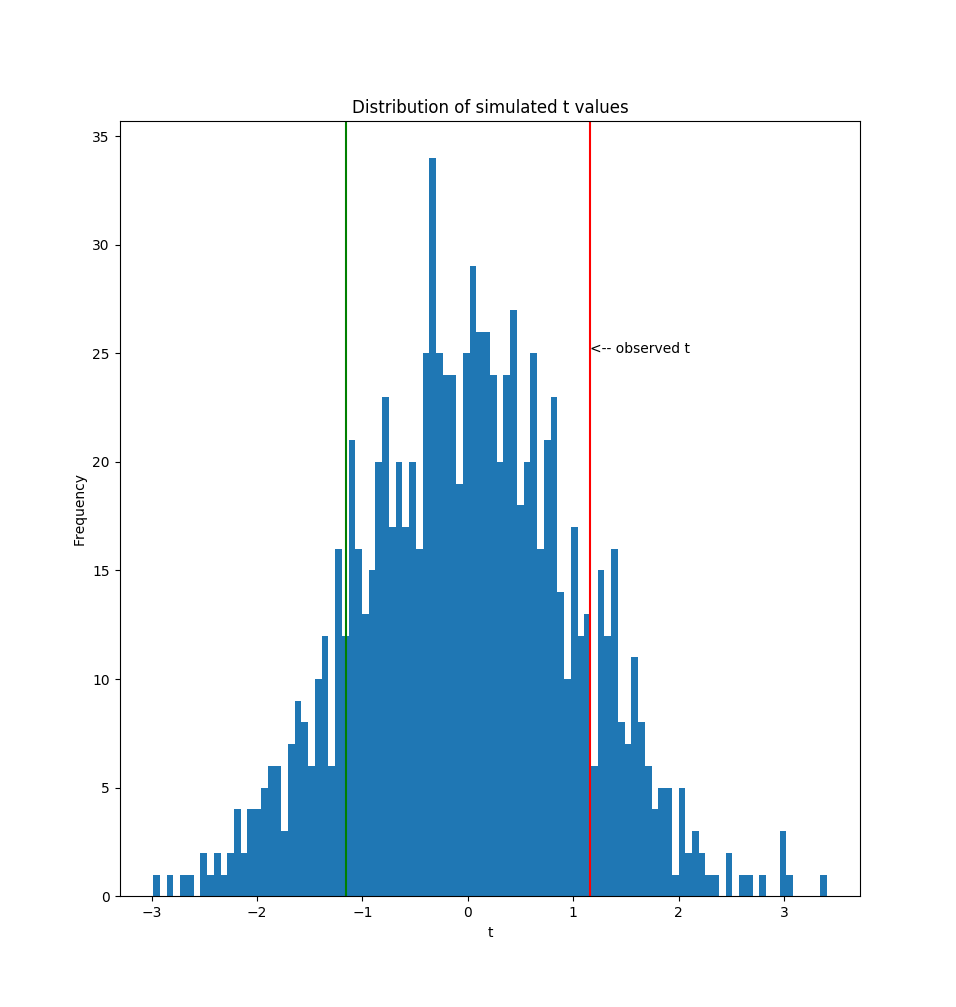
\includegraphics[width=\linewidth]{./Figure2.png}
                 \caption{This is another two side bell-like-curve that is created with the t simulated values. t obsevered stay the same as before.}
                \label{figure:graph2}
                 \end{figure} 
                

                  \begin{figure}
                 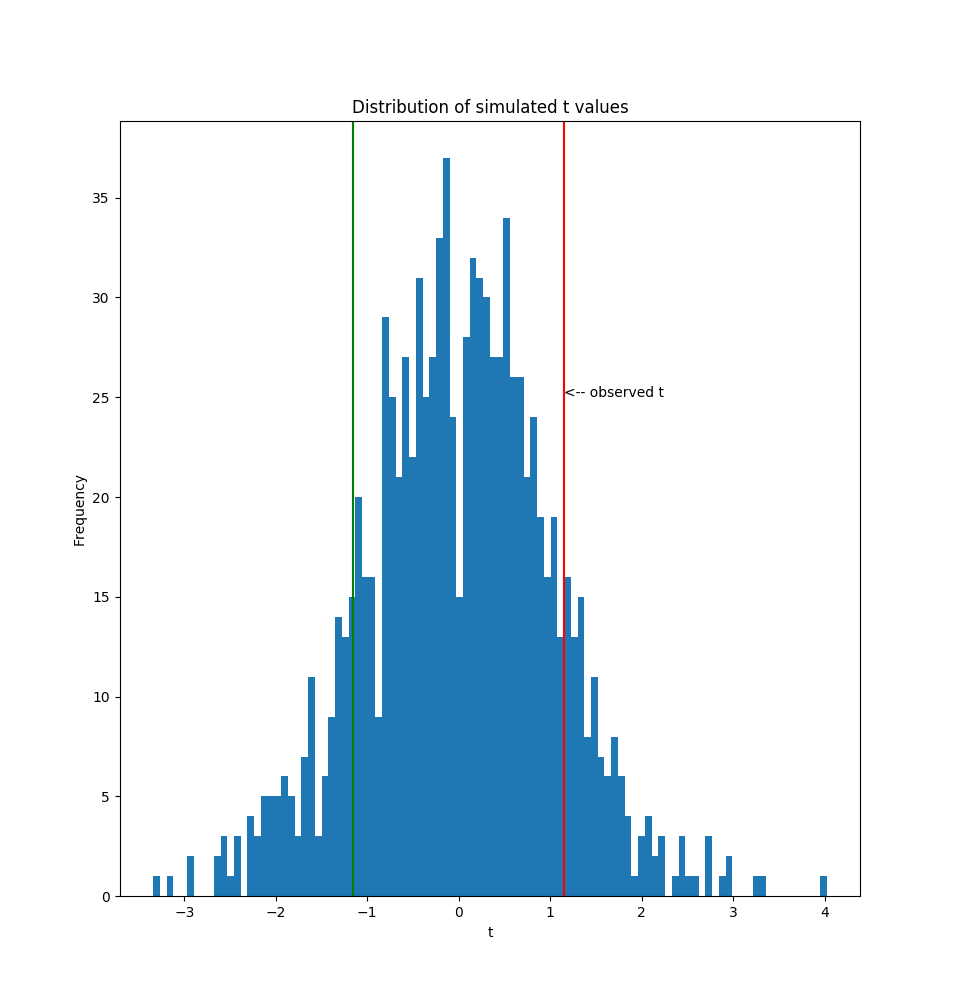
\includegraphics[width=\linewidth]{./Figure3.png}
                 \caption{This is another two side bell-like-curve that is created with the t simulated values. t obsevered stay the same as before.}
                \label{figure:graph3}
                \end{figure} 
  \part{2.D}
     Based on the result there is at least 7030 genes have a value that is greater then .025 and less than this value -.025. so that means that there is about a 98 $\%$ of these genes that show with at least alternative points. 
  \part{2.E}
 The permuntation test results has a varity of randomized assorted ways to extrapolate the data one of which is that the one tailed has about 33934000-3936999 and is closely linked to about 45 $\%$  of the total data. If we use the both tails to compare the results, I would get anywhere around this 482000-488999 of the data was less than .025. Therefore the data  is about a 6.7-6.8 $\%$ of finding that the numbers are within a relative close margin of data to both 2.5 $\%$ without understating the data.  Then the regular two-sample T-test in which doesn't vary and ulitmatlely it has a 7030 genes that is closer to the out of 7128 genes that was read throught proves that when looking at the ends it allows you to receive that data at about 1.375, and in which is undetstates the data that there is about  2.5 $\%$ of it actual within that slot.  

\end{document}

